\begin{frame}{\linux:von Grund auf}{Image auf SD-Karte}
 \begin{itemize}
  \item Bootloader
  \item Kernel
  \item RootFS
 \end{itemize}
\end{frame}

\begin{frame}{The Big Picture}
\begin{center}
 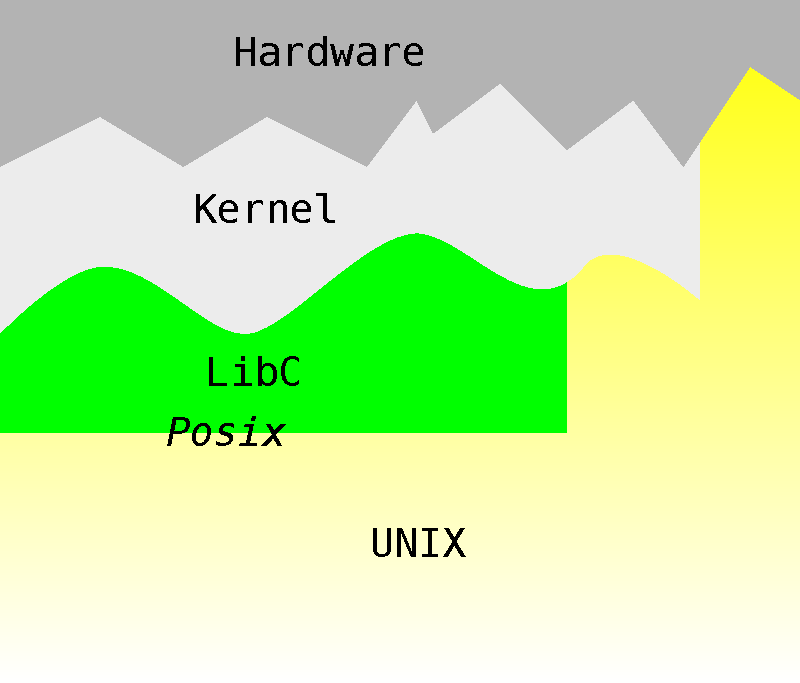
\includegraphics[height=0.875\textheight]{layers.pdf}
\end{center}
\end{frame}

\subsection{Partitionen}
\begin{frame}{Image: 2 Partitionen}{Siehe \cod{3.5-partitions}}
 \begin{description}[Partition 1: p1]
  \item[Partition 1: p1] \cod{vfat} Bootloader, kernel 
  \item[Partition 2: p2] \cod{ext4} RootFS
  \item[Befehle] auf dem \host
  \begin{itemize}
   \item \cod{fdisk} 
   \item \cod{mkfs.vfat}
   \item \cod{mkfs.ext4}
  \end{itemize}
 \end{description}
\end{frame}

\subsection{Boot/Kernel}
\begin{frame}{Herstellung}{Teil 1: wenig files}
 \begin{description}[toolchain-bare:]
  \item[toolchain-bare:] Siehe \cod{17-build/tools/\{binutils.sh | gcc-bare.sh\}}
  \item[u-boot:] Siehe \cod{4-uboot}
  \begin{itemize}
   \item \cod{MLO}
   \item \cod{u-boot.img}
  \end{itemize}
  \item[kernel:] Siehe \cod{5-kernel}
  \begin{itemize}
   \item \cod{zImage}
   \item \cod{am335x-boneblack-wireless.dtb}
  \end{itemize}
 \end{description}
\end{frame}

\newcommand{\targetRoot}[1]
{
{
\footnotesize
\setlength{\DTbaselineskip}{0.875em}
\dirtree{%
.1 #1.
.2 bin.
.2 dev.
.2 etc.
.2 home.
.2 lib.
.2 linuxrc.
.2 made-{\em yyyy-mm-dd}.
.2 proc.
.2 sbin.
.2 share.
.2 sys.
.2 usr.
}
}
}

\subsection{RootFS}
\begin{frame}{Herstellung RootFS}{\host\ - SD-Card - Target(\targetS)}
\begin{columns}
\begin{column}{0.3\textwidth}
 \host
 
 \targetRoot{{\em path-to-target-root}}
\end{column}
\begin{column}{0.3\textwidth}
 SD-Card
 
 \targetRoot{{\em path-to-sd-card}}
\end{column}
\begin{column}{0.3\textwidth}
 \targetS
 
 \targetRoot{/}
\end{column}
\end{columns}
\begin{block}{Transport}
 \vspace{-2mm}
 \begin{description}[SD-Card $\to$ \targetS:]
  \item[\host $\to$ SD-Card:] \cod{rsync -av {\em path-to-target-root} {\em path-to-sd-card}}
  \item[SD-Card $\to$ \targetS:] einstecken
  \item[SD-Card $\to$  \host:]\cod{rsync -av {\em path-to-sd-card} {\em path-to-target-root}}
 \end{description}
\end{block}
\end{frame}


\begin{frame}{Herstellung}{Teil 2: RootFS}
 \begin{description}[toolchain] 
  \item[LibC] Siehe \cod{17-build/tools/glibc.sh}
  \item[toolchain] \cod{17-build/tools/gcc.sh}
  \item[\unix] Verschiedene {\em flavours}
  \begin{itemize}
   \item minimal: Siehe \cod{19-minimal}
   \item busybox: Siehe \cod{17-build/tools/busybox.sh}
  \end{itemize}
 \end{description}
\end{frame}

\begin{frame}{Ausbau}
 \begin{description}[WLAN]
  \item[ssh]  Siehe \cod{17-build/tools/openssh.sh}
  \item[WLAN] Siehe \cod{6-assembly}
  \item[init] Siehe \cod{6-assembly}
 \end{description}
\end{frame}
